\documentclass[11pt,a4paper]{article}
\usepackage[margin=25mm]{geometry}
\usepackage[T1]{fontenc}
\usepackage{lmodern,microtype}
\usepackage{amsmath,amssymb,graphicx,booktabs,tabularx}
\usepackage{caption,float,placeins,enumitem,xcolor,hyperref,fancyhdr}
\hypersetup{colorlinks=true,linkcolor=blue!45!black,urlcolor=blue!45!black,citecolor=blue!45!black,pdftitle={Identifying Financial Market States: An Independent Reproduction and Critical Evaluation}}
\setlength{\parskip}{0.30em}
\setlength{\parindent}{0pt}
\setlist[itemize]{topsep=0.2em,itemsep=0.1em}
\pagestyle{fancy}
\fancyhf{}
\fancyhead[L]{\small Financial market states}
\fancyhead[R]{\small Reproduction and evaluation}
\fancyfoot[C]{\thepage}
\renewcommand{\headrulewidth}{0.3pt}
\graphicspath{{../munik/analysis/notebook_paper_v2/}}
\title{Identifying Financial Market States\\[0.25em]\large An Independent Reproduction and Critical Evaluation of M\"unnix et al.\ (2012)}
\author{Independent Data Mining Research Project\\Sharif University of Technology}
\date{2026}
\begin{document}
\maketitle
\begin{abstract}
We reconstruct the daily-data workflow of M\"unnix et al., \emph{Identifying States of a Financial Market} (2012), using historical stock prices from 1992--2010. After auditing 300 stock files across ten sectors, 296 stocks remain in the final correlation analysis. We compute locally normalized daily returns, 114 disjoint two-month correlation matrices, and a complete top-down clustering tree. At the article's stopping threshold of 0.1465, this dataset yields two states; an explicitly calibrated threshold of 0.1301746 yields eight. Mean silhouette scores are 0.278 and 0.047, respectively. We also compute 4,733 daily rolling windows and their full matrix-distance map, visualize sector structure, state evolution, the 2008 crisis distribution, the complete clustering tree, and a largest-eigenvalue alternative. The eight-state partition provides an informative comparison, but its count was selected on these data and is not an independent replication of the article's eight states. We document the data choices, implementation, discrepancies, and limits of inference so that the reported results can be reviewed and reproduced.
\end{abstract}
\setcounter{tocdepth}{1}
\tableofcontents
\newpage

\section{Introduction and research question}
Financial markets are not stationary: dependence between stocks can change substantially over time. A single correlation matrix estimated over the full sample can therefore hide periods of relative calm, transitions, and collective movement. M\"unnix et al.\ \cite{munnix2012} proposed treating the correlation structure within a short window as a market state, comparing windows by matrix differences, and grouping recurring structures with top-down clustering.

This project asks how much of the article's empirical workflow can be reconstructed from the available daily price files, and how sensitive the number and quality of the resulting states are to data choices and the clustering threshold. It began as a Data Mining seminar reproduction and developed into an evaluation of whether obtaining a desired number of clusters also gives a convincing partition. Our contributions are a documented Python pipeline, comparable visualizations, and a transparent account of the disagreement with the published eight-state result.

\section{The original study and the scope of this reproduction}
The article studies S\&P 500 stocks over 1992--2010. Its principal daily analysis uses arithmetic returns, 13-observation local normalization, two-month correlation matrices, an entrywise matrix-distance measure, and top-down clustering. The authors report eight characteristic states at a stopping threshold of 0.1465. Their figures show a time-by-time similarity map, sector-sorted state matrices, deviations from the overall matrix, a state timeline, crisis-period correlation histograms, and the full division tree \cite{munnix2012}.

The article also examines 2007--2010 with intraday NYSE TAQ observations: one-hour returns sampled every minute and one-week correlation windows. Our files contain daily prices only. Our corresponding 2007--2010 panel is a \emph{daily-data zoom}, not a reconstruction of the intraday panel. Exact historical index membership and the article's original price series have not been established from our supplied files.

\section{Data provenance and cleaning}
\subsection{Inputs and calendar alignment}
The local input has 300 individual stock CSV files organized into ten sector folders and a supplied trading-date reference. The main analysis uses adjusted close. The reference calendar has 4,789 trading dates from 2 January 1992 through 31 December 2010. Original files are preserved; cleaned outputs are written separately. We parse dates and numeric values, check duplicate and invalid observations, restrict to the reference calendar, sort chronologically, and align stocks in a date-by-ticker table. We do not interpolate, forward-fill, or winsorize prices. Zero-volume rows remain because the correlation analysis uses prices, not volume; 286 such rows were flagged in the source-file audit.

\begin{table}[htbp]\centering
\caption{Data audit and analysis universe. Missing prices refer to the aligned 300-stock panel.}\label{tab:data}
\begin{tabular}{@{}p{0.60\linewidth}r@{}}\toprule
Quantity & Value \\ \midrule
Raw stock files / sectors & 300 / 10 \\
Reference trading dates & 4,789 \\
Missing aligned adjusted-close prices & 558 \\
Stocks with complete price history & 297 \\
Stocks in final correlation analysis & 296 \\
Daily arithmetic return observations & 4,788 \\
Observations after 13-point warm-up & 4,776 \\
Disjoint two-month terms & 114 \\
Eligible daily rolling windows & 4,733 \\
\bottomrule\end{tabular}\end{table}

MAC lacks 554 calendar dates, PLL lacks three, and ADI lacks one, totaling 558 missing cells. PLL also contains 53 observations outside the reference calendar, which are excluded from the aligned panel. Removing the three incomplete-history stocks leaves 297.

Local normalization reveals a separate problem: PBCT has eight dates in December 1993 for which all 13 returns in the normalization window are zero. Its local standard deviation is zero. We exclude PBCT from the correlation universe instead of inventing values or dropping those dates market-wide, leaving a fixed 296-stock universe. This is our explicit implementation choice, not a rule stated by the article. Complete historical prices do not prove continuous S\&P 500 membership, and low two-decimal adjusted prices could introduce rounding effects. Both issues merit further audit.

\section{Methods and implementation}
\subsection{Returns, local normalization, and windows}
For stock $i$ on consecutive trading dates we use the arithmetic return
\begin{equation}r_i(t)=\frac{S_i(t+1)-S_i(t)}{S_i(t)}.\label{eq:return}\end{equation}
The return is labeled by its starting date $t$. We then compute, independently for each stock,
\begin{equation}
\widetilde r_i(t)=\frac{r_i(t)-\langle r_i\rangle_{t,13}}
{\sqrt{\langle r_i^2\rangle_{t,13}-\langle r_i\rangle_{t,13}^{,2}}},
\label{eq:normalize}\end{equation}
where the averages cover the 13 most recent returns including the current observation. Population variance is used in this local expression. The first 12 returns cannot be normalized; a zero denominator is detected explicitly.

For clustering we use six non-overlapping calendar terms per year: January--February through November--December, matching the article's full-tree term definition. This gives 114 terms over 19 years. The first term contains 29 usable normalized returns after warm-up; later terms generally have about 40--44. For the high-resolution similarity map, a separate trailing two-calendar-month window advances one trading date at a time. The two schedules serve different analyses.

\subsection{Correlation matrices and matrix distance}
Within each window, we calculate the Pearson correlation matrix $C^{(a)}$ of the 296 normalized stock-return series. For two windows $a$ and $b$, the matrix distance is
\begin{equation}
d(a,b)=\frac{1}{N^2}\sum_{i=1}^{N}\sum_{j=1}^{N}
\left|C_{ij}^{(a)}-C_{ij}^{(b)}\right|,\qquad N=296.
\label{eq:distance}\end{equation}
The diagonal contributes zero for valid correlation matrices but remains in the $N^2$ scaling. For storage and speed, the code uses the upper triangle with weight $1/N^2$ on diagonal entries and $2/N^2$ off the diagonal. This is algebraically equivalent to Equation~\eqref{eq:distance}. The 114 disjoint matrices produce a symmetric $114\times114$ distance matrix.

\subsection{Top-down clustering and threshold choice}
All 114 matrices start in one node. At each split, the implementation considers every pair of member matrices as initial centers, assigns matrices to the nearer center, recomputes arithmetic-mean centers, and repeats until labels stop changing. Among converged initial pairs, it selects the division with the smallest mean \emph{squared scalar matrix distance} to assigned centers. A node continues splitting while its average member-to-center distance exceeds the threshold. Splitting down to singletons produces 227 nodes and 114 leaves.

We interpret the article's $\zeta^{(L)}$ assignment distance as Equation~\eqref{eq:distance}. The published methods do not fully specify this notation or every tie-handling detail. The code makes these choices explicit and rejects empty groups, cycles, or non-convergence. This is a close computational reconstruction, not a claim of identical historical software.

First we cut the fitted tree at the article's $\tau=0.1465$. The threshold interval yielding exactly eight leaves on \emph{our} tree is $0.1297764<\tau<0.1305729$; its midpoint $\tau=0.1301746$ is used for the eight-state visual comparison. That midpoint was selected after seeing the tree and is not an independently selected optimum.

\subsection{Diagnostics and computational strategy}
For each state we average member correlation matrices; the overall mean gives equal weight to each two-month window. State-minus-overall matrices share this reference. Diagnostics include mean off-diagonal correlation, within- and between-sector means, energy-to-other-sector correlation, negative-pair fraction, and mean silhouette score. Silhouette uses the same matrix-distance geometry as the clustering. It is an internal measure of separation, not proof of economic validity.

The full daily analysis has 4,733 eligible windows, from 20 March 1992 through 30 December 2010, and $4{,}733\times4{,}732/2=11{,}198{,}278$ distinct pairs. Double-precision features and distances are held in disk-backed arrays; Numba-compiled kernels compute pairwise distances. Completion flags allow resuming an interrupted run. We checked finite non-negative values, symmetry, and a zero diagonal. The completed distance matrix is $4{,}733\times4{,}733$ with maximum observed distance 0.6597. An alternative summary uses the largest correlation-matrix eigenvalue and its absolute difference across dates, as discussed in the article.

\section{Results}
\subsection{Daily similarity structure}
Figure~\ref{fig:daily} shows the complete daily matrix-distance map and a magnified 2007--2010 daily subset. Light cells indicate similar correlation structures; darker cells indicate larger differences. Persistent bands and crisis-era contrasts show that market dependence changes over time and that some structures recur. The right panel has its own color scale for readability and is a subset of the same daily distance matrix. It is not the article's intraday panel.

\begin{figure}[htbp]\centering
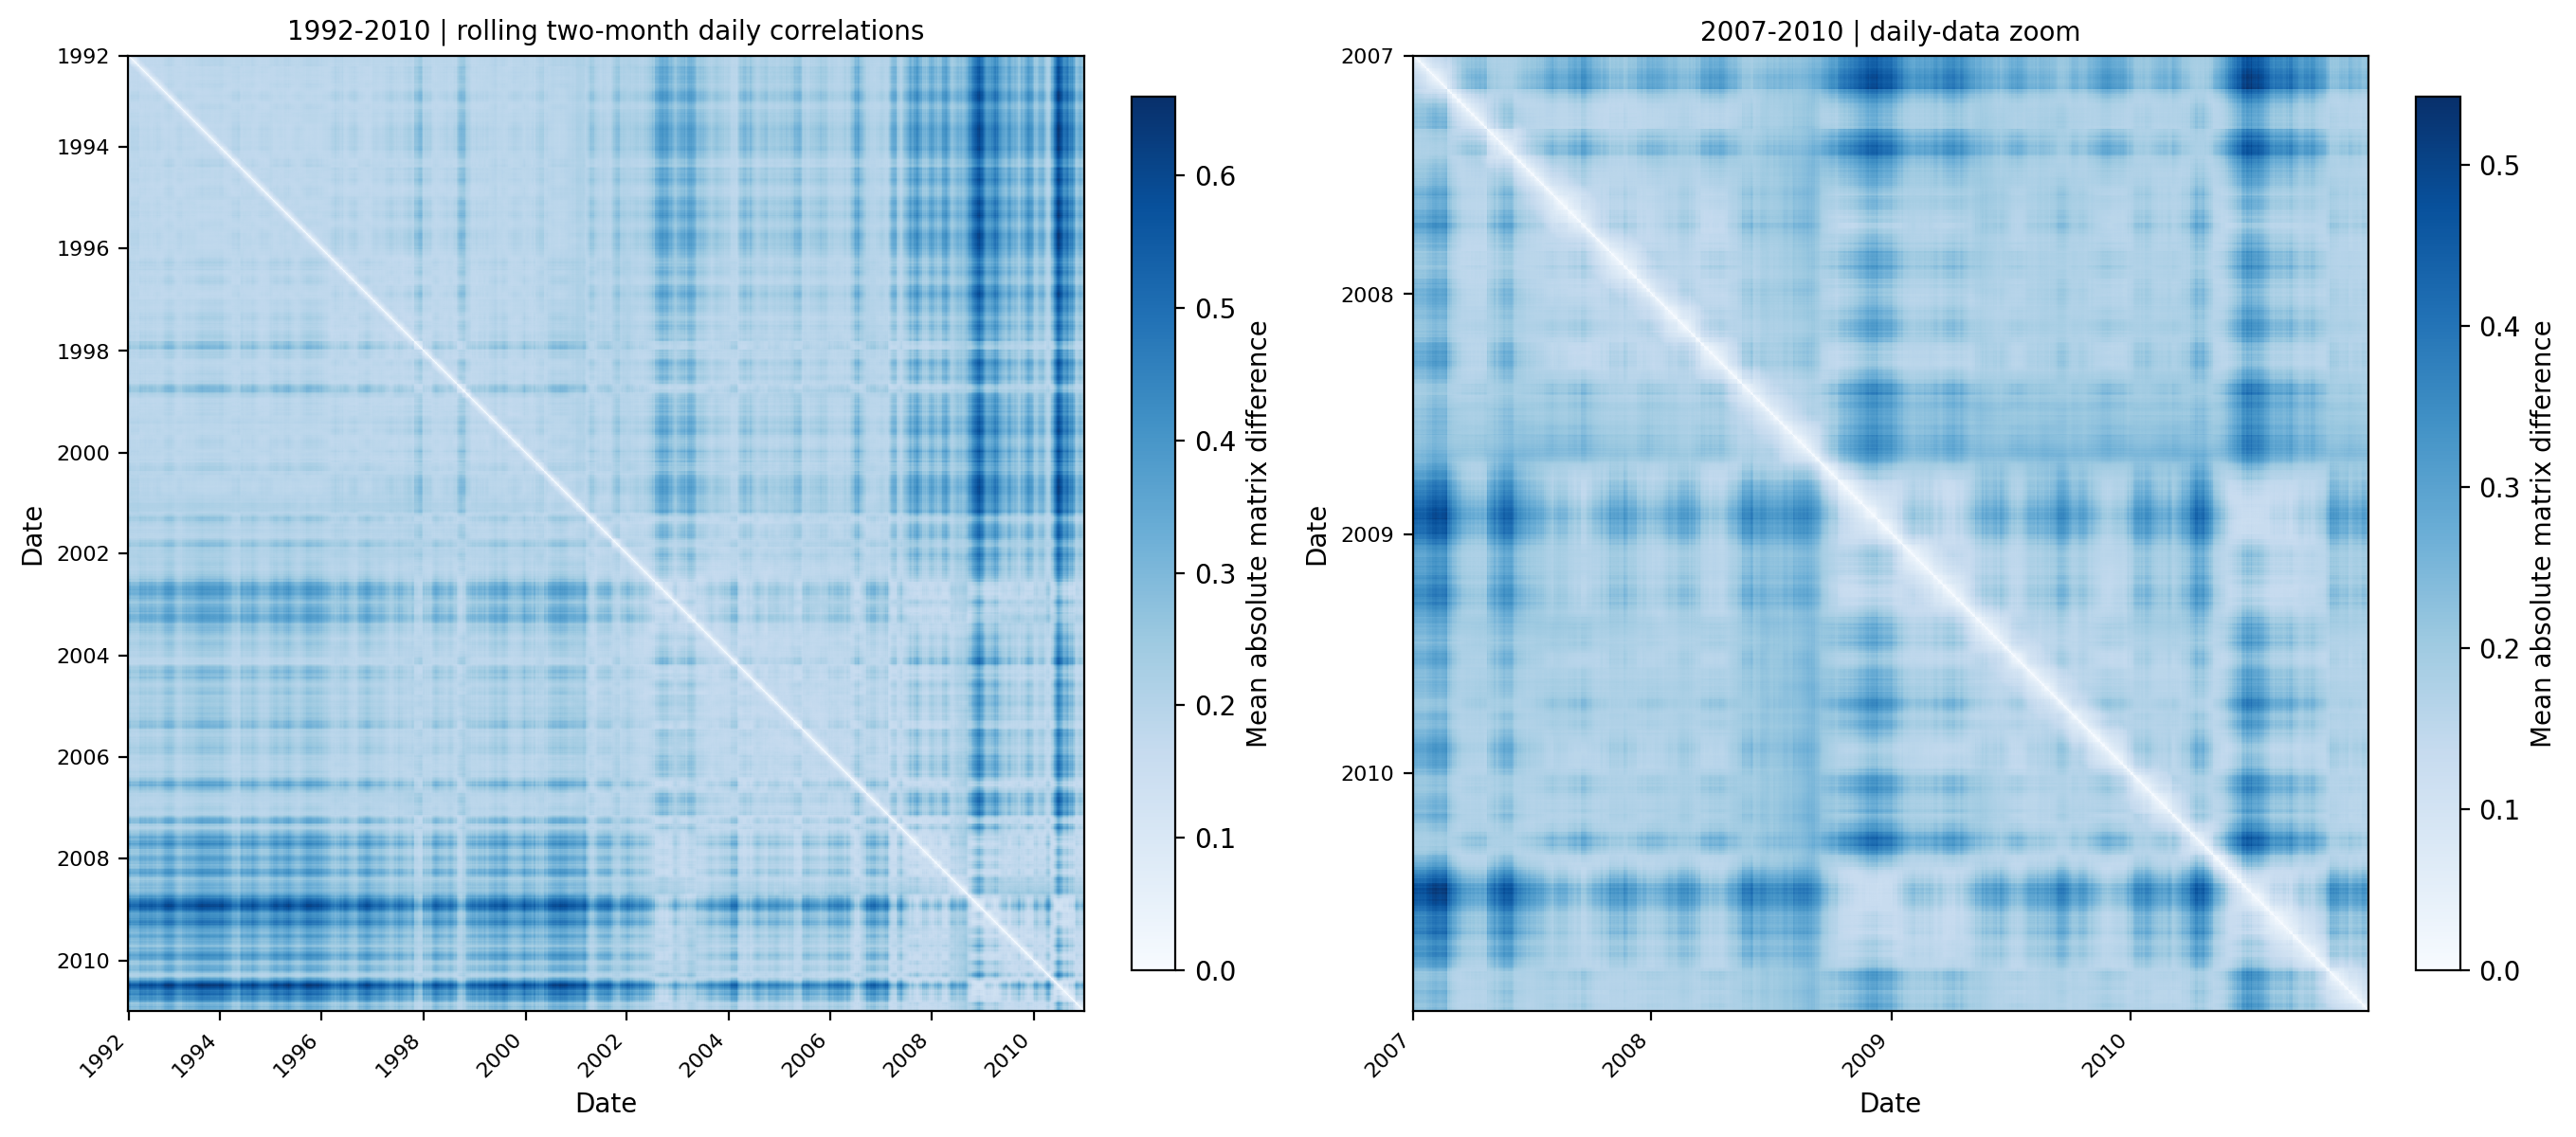
\includegraphics[width=0.98\linewidth]{figure1_daily_rolling_similarity.png}
\caption{Our daily-data counterpart to the article's Figure 1. Left: all 4,733 trailing two-month daily windows. Right: daily-data zoom for 2007--2010. The original right panel used intraday TAQ data, unavailable here.}\label{fig:daily}
\end{figure}

The 114 disjoint-window distances in Figure~\ref{fig:terms} show the lower-resolution geometry used for clustering. These separated terms should not be confused with the 4,733 overlapping daily windows.
\begin{figure}[htbp]\centering
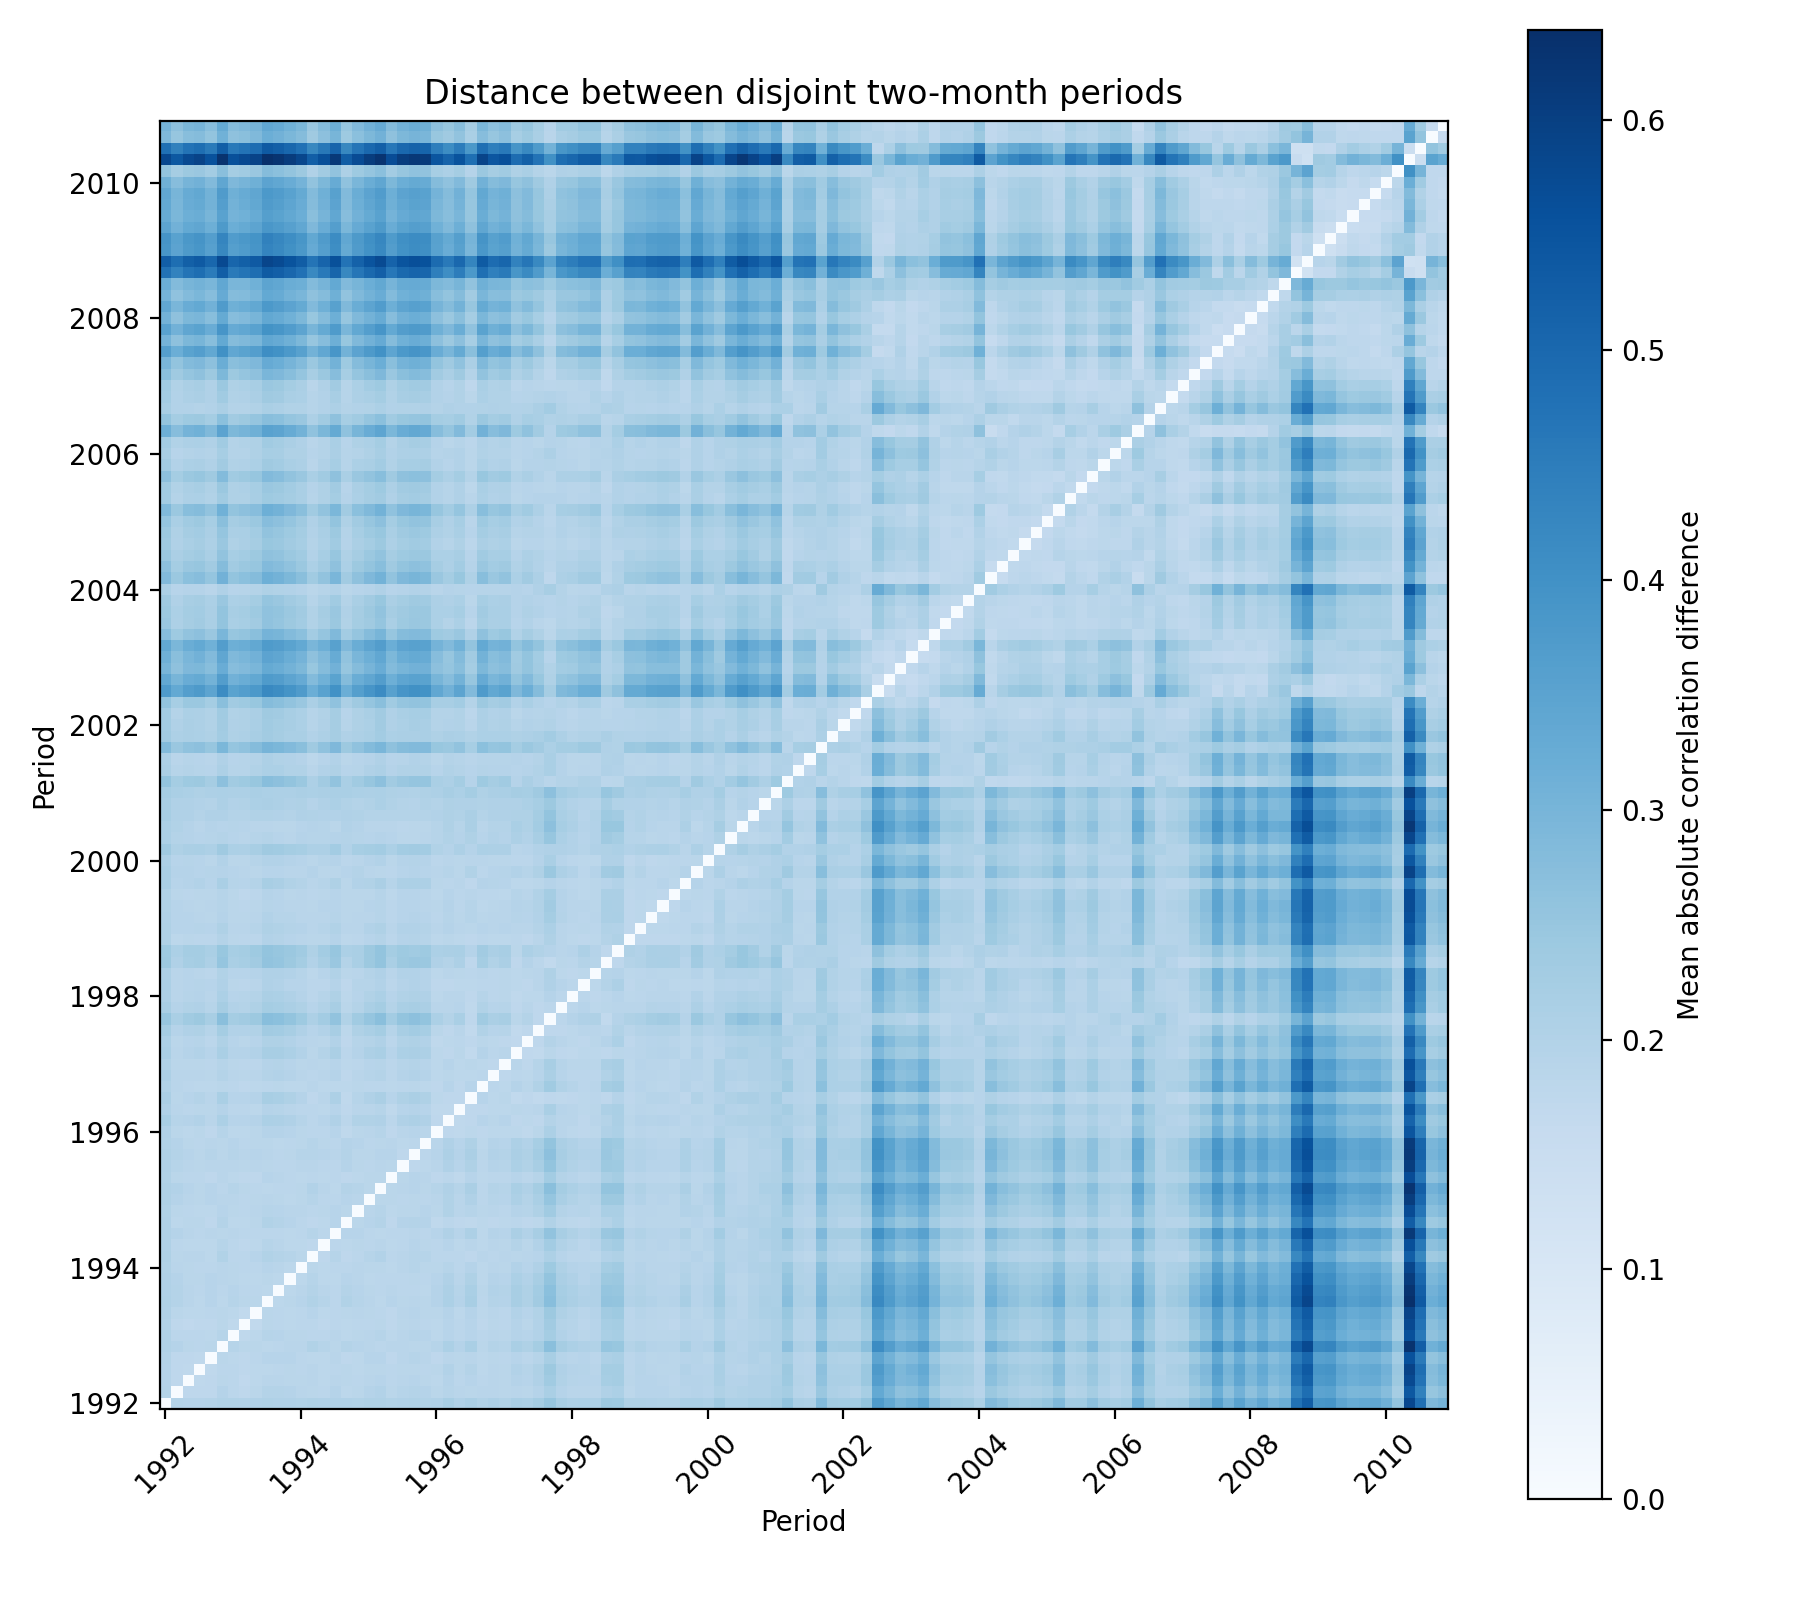
\includegraphics[width=0.79\linewidth]{disjoint_period_distances.png}
\caption{Distances among 114 non-overlapping two-month correlation matrices used for state clustering.}\label{fig:terms}
\end{figure}

\FloatBarrier
\subsection{Two states at the published threshold; eight after calibration}
The published threshold 0.1465 yields \textbf{two states} on our data. The calibrated midpoint 0.1301746 yields eight groups. These are cuts of the same fitted tree, not independently estimated models. The mean silhouette drops from 0.2775 for two states to 0.0474 for eight, suggesting weaker separation of the additional divisions under our matrix distance. This does not establish that the market has exactly two true states.

\begin{table}[htbp]\centering
\caption{Threshold sensitivity on the same 114-window tree. The eight-state threshold was fitted to the desired count.}\label{tab:threshold}
\begin{tabular}{@{}p{0.48\linewidth}rrr@{}}\toprule
Tree cut & Threshold & States & Mean silhouette \\ \midrule
Published article threshold & 0.1465000 & 2 & 0.2775 \\
Calibrated eight-state midpoint & 0.1301746 & 8 & 0.0474 \\
\bottomrule\end{tabular}\end{table}

Figure~\ref{fig:states} displays the eight calibrated centers, their relationship within the fitted tree, and the overall mean matrix. Stocks follow the article's sector order: E, M, I, CD, CS, H, F, IT, C, U. We number states by first appearance in our timeline. The labels cannot be matched directly to the paper's numbered states. Figure~\ref{fig:diff} subtracts the same window-weighted overall mean matrix from each center to highlight sector-specific departures.

\begin{figure}[htbp]\centering
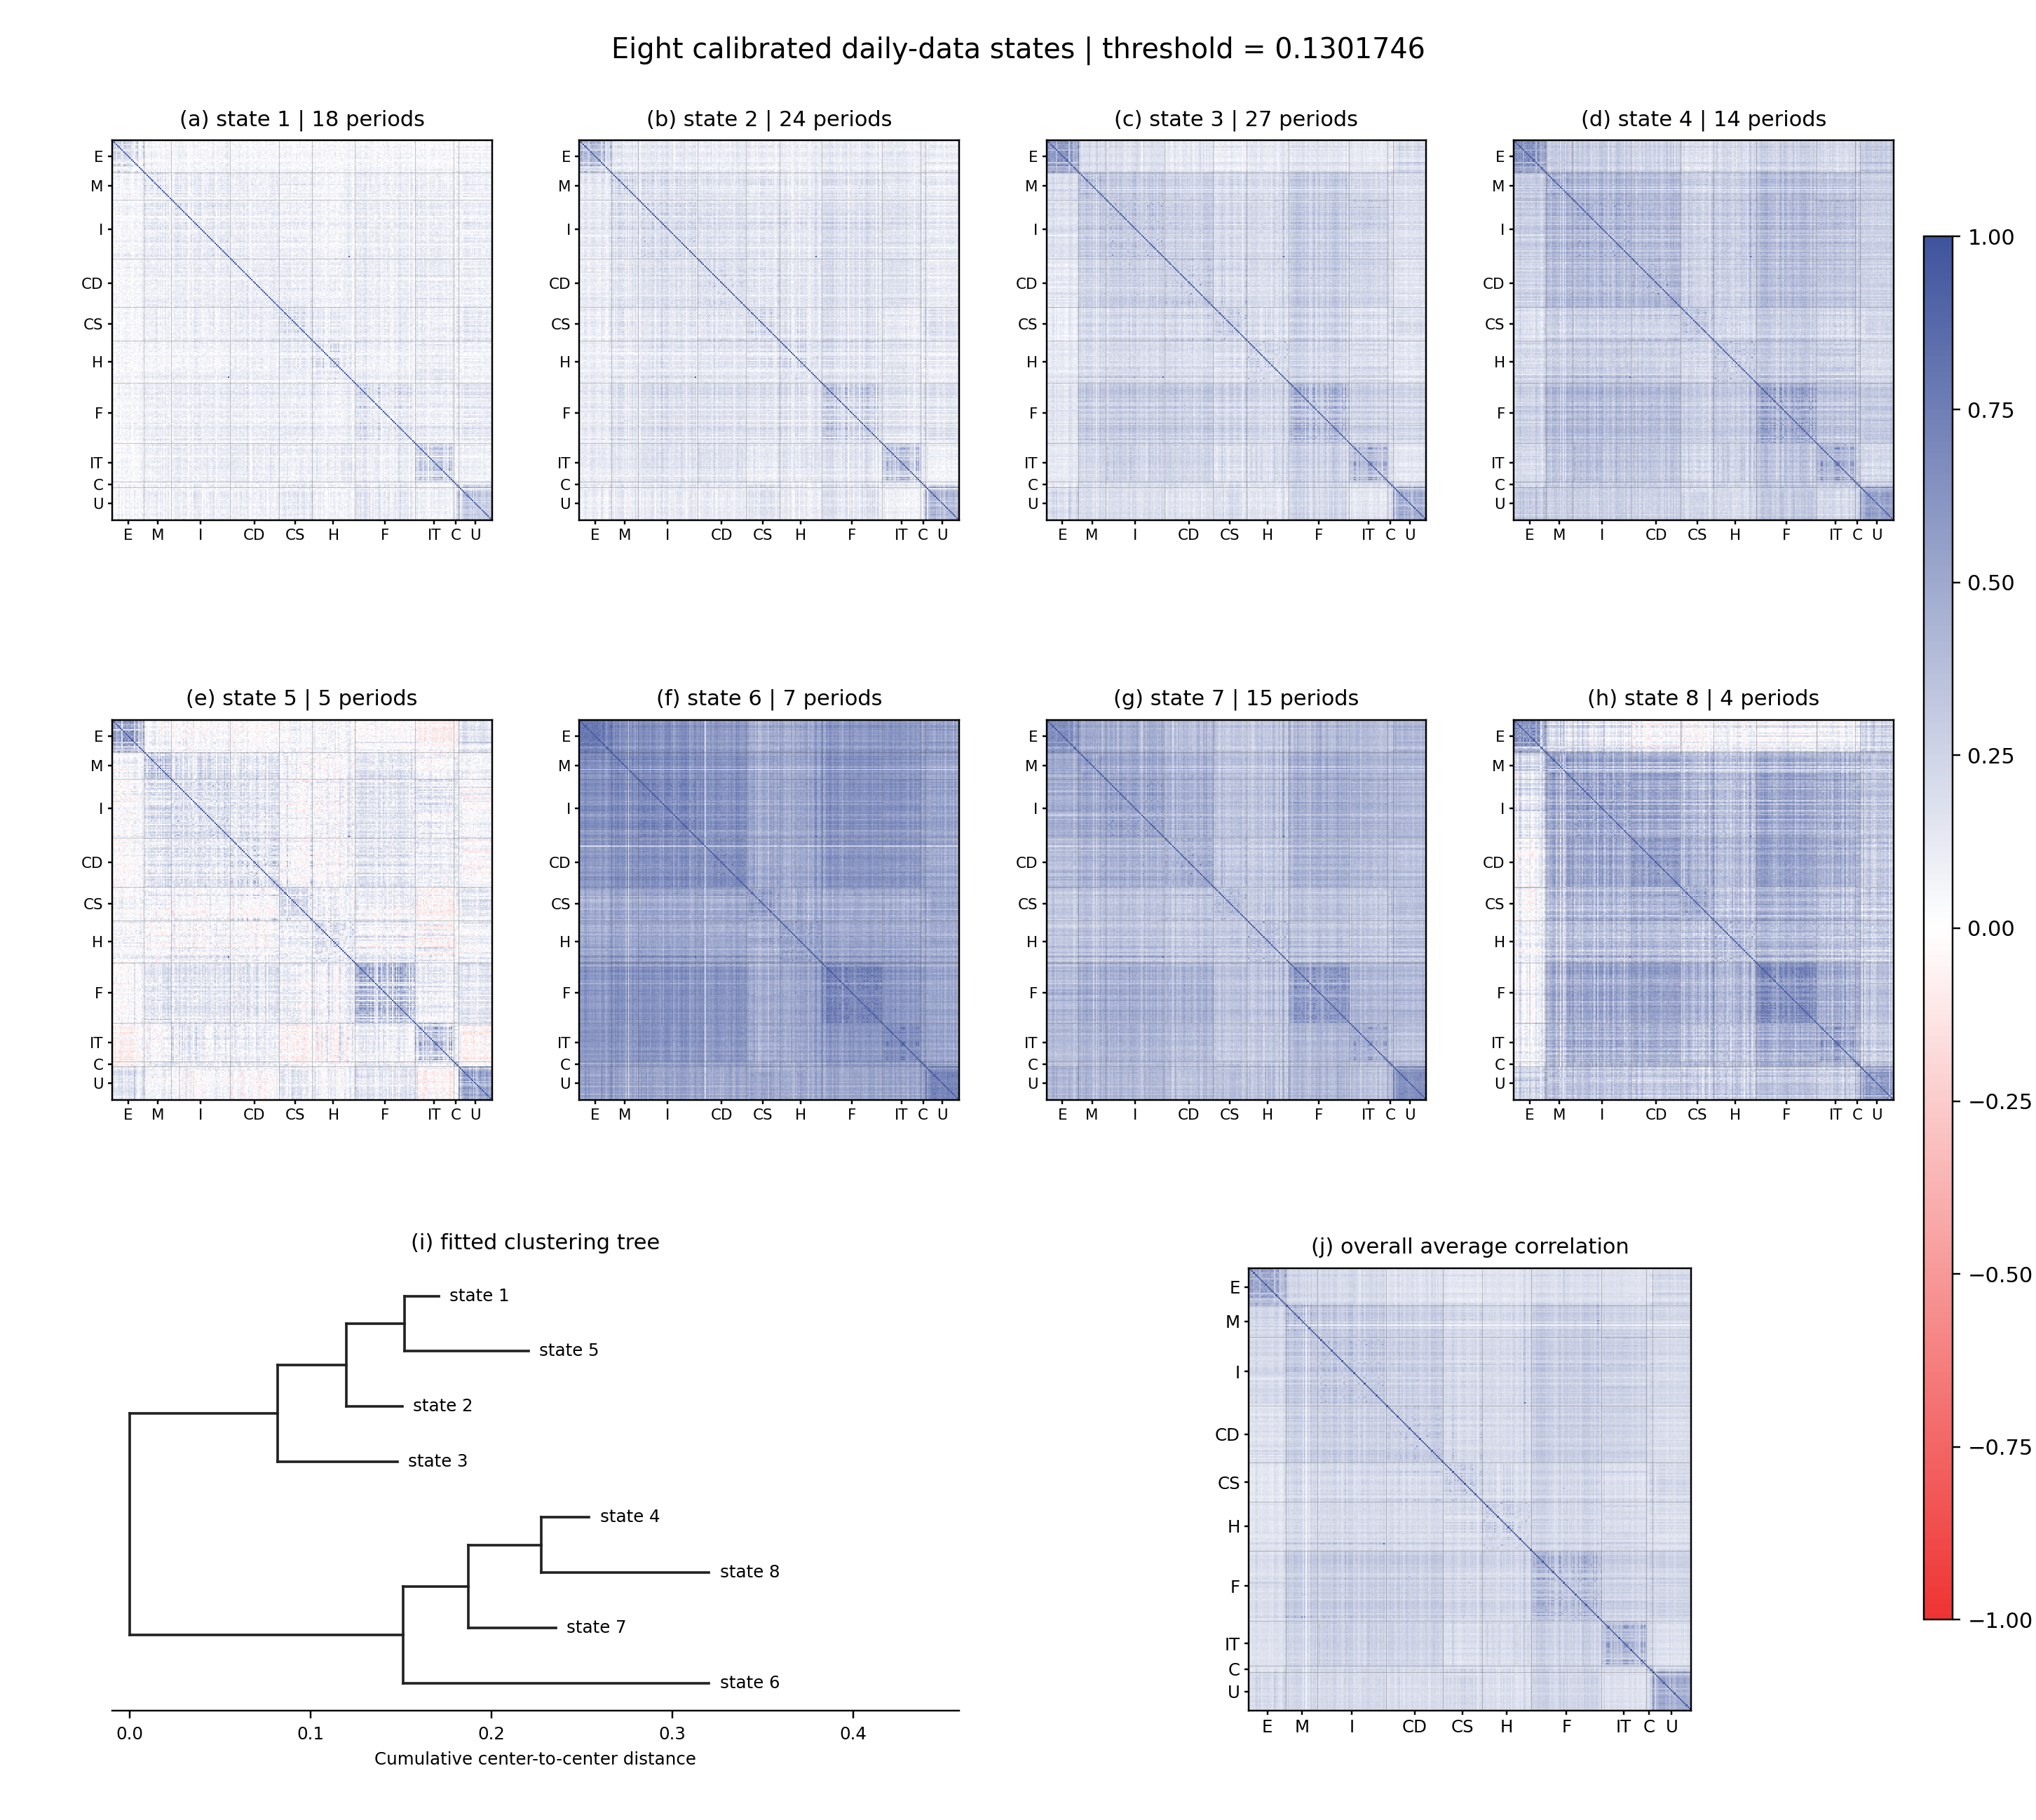
\includegraphics[width=0.98\linewidth]{figure2_states.png}
\caption{Eight calibrated state centers, their fitted-tree relationship, and the overall matrix. A structural counterpart to the article's Figure 2, with state numbering specific to our dataset.}\label{fig:states}
\end{figure}
\begin{figure}[htbp]\centering
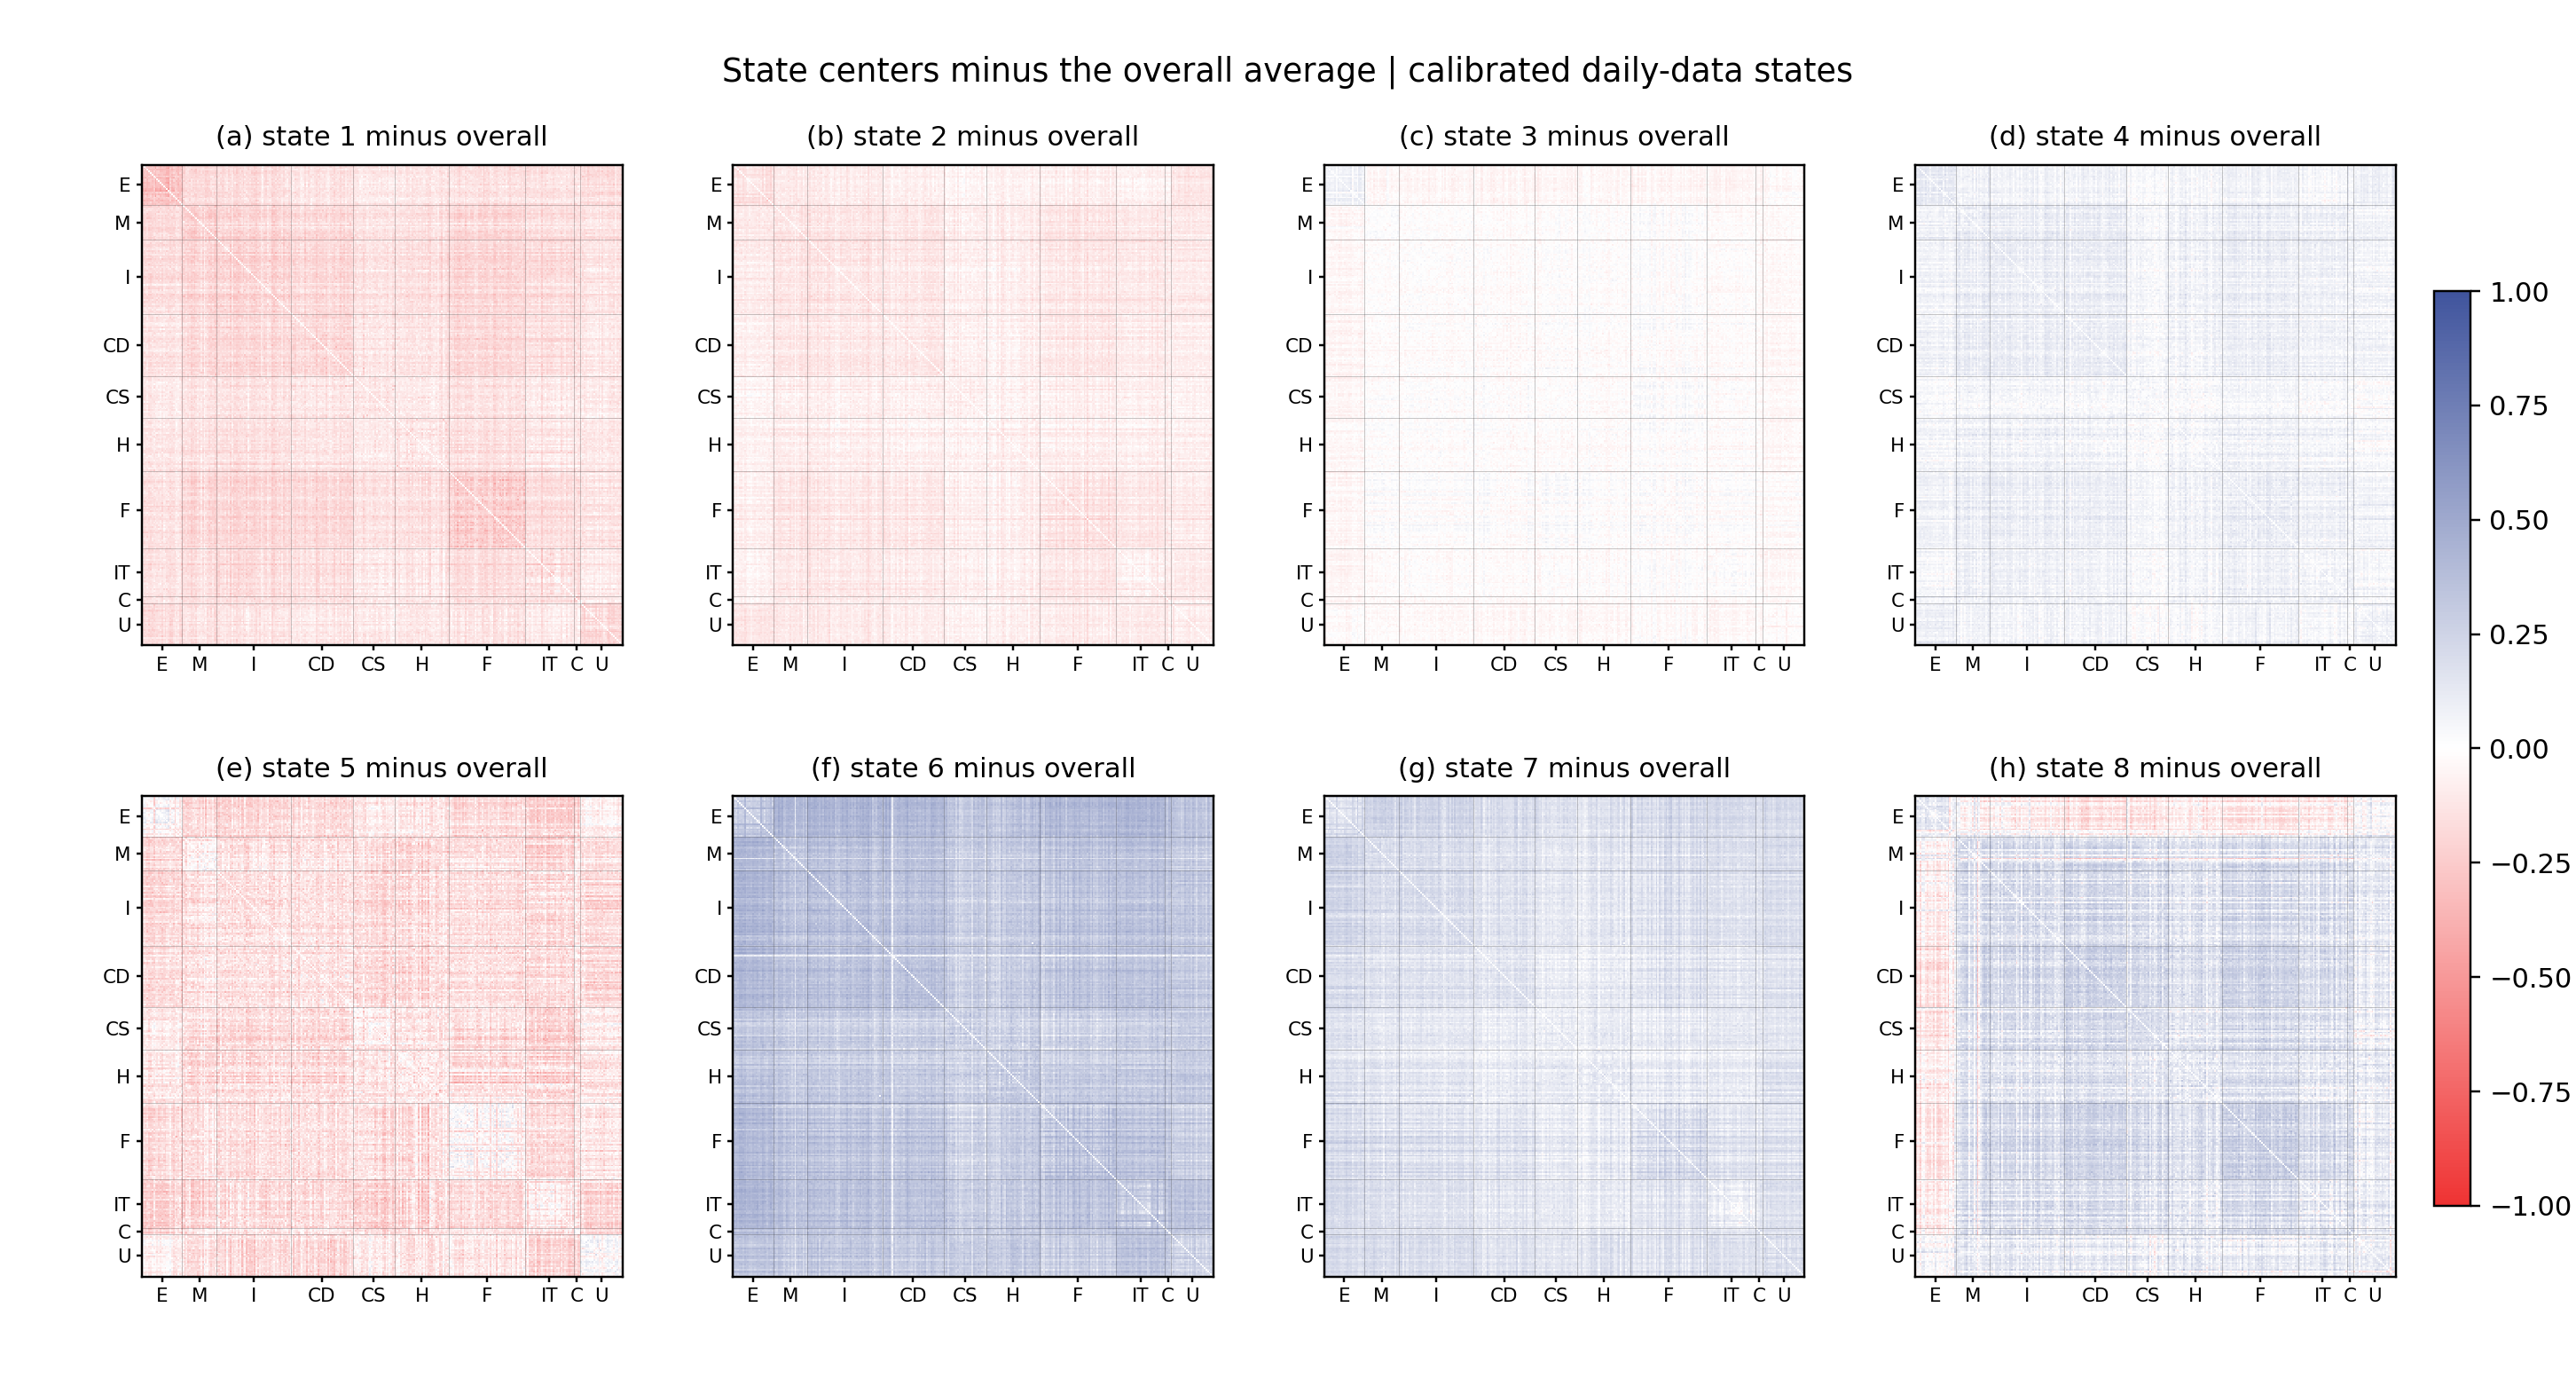
\includegraphics[width=0.98\linewidth]{figure3_differences.png}
\caption{State centers minus the window-weighted overall matrix, corresponding in purpose to the article's Figure 3. All panels use a shared color scale.}\label{fig:diff}
\end{figure}
\FloatBarrier

\begin{table}[htbp]\centering
\caption{Selected diagnostics of the eight calibrated states. Correlations are means across off-diagonal stock pairs; negative pairs are percentages.}\label{tab:states}
\small\begin{tabular}{@{}rrrrrr@{}}\toprule
State & Terms & Mean $C$ & Within sector & Energy to others & Negative pairs (\%) \\ \midrule
1 & 18 & 0.089 & 0.136 & 0.048 & 5.73 \\
2 & 24 & 0.146 & 0.218 & 0.106 & 0.57 \\
3 & 27 & 0.222 & 0.323 & 0.147 & 0.05 \\
4 & 14 & 0.306 & 0.412 & 0.246 & 0.01 \\
5 &  5 & 0.093 & 0.241 & 0.034 & 20.69 \\
6 &  7 & 0.559 & 0.645 & 0.571 & $<0.01$ \\
7 & 15 & 0.396 & 0.491 & 0.393 & 0.00 \\
8 &  4 & 0.363 & 0.510 & 0.114 & 3.58 \\
\bottomrule\end{tabular}\end{table}

The state matrices show a wide range of dependence, from weakly connected states 1 and 5 to strongly correlated state 6. State 5 has the largest negative-pair fraction in this cut. State 8 has relatively weak energy-to-other-sector correlation compared with its overall mean. These are descriptions of the calibrated groups; assigning the article's crisis-state names to them would require separate, documented matching.

\FloatBarrier
\subsection{Temporal sequence and the 2008 crisis}
Figure~\ref{fig:timeline} places the calibrated labels on the calendar. A state can recur after the market has moved through others. States 6 and 7, which have relatively high mean correlations, occur in later periods including the 2008--2009 episode. The two-month resolution smooths fast transitions. Our state 8 occurs in four terms and is not identical to the article's state 8.

\begin{figure}[htbp]\centering
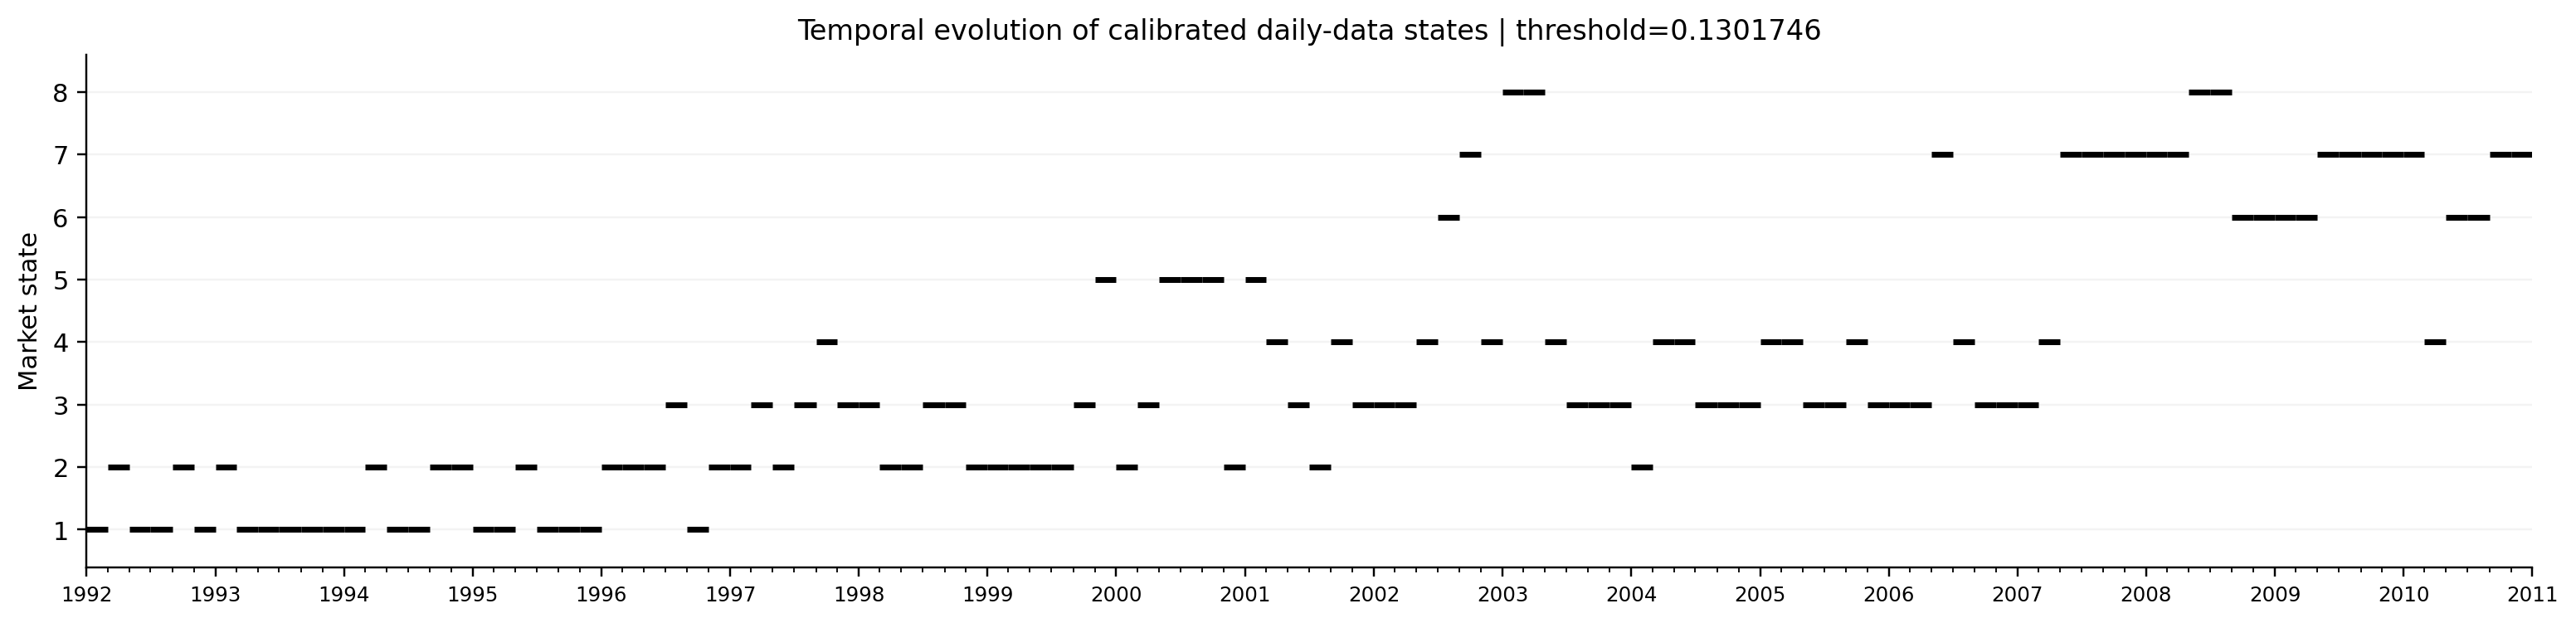
\includegraphics[width=0.96\linewidth]{figure4_timeline.png}
\caption{Time sequence of eight calibrated states across 114 disjoint two-month terms, analogous to the article's Figure 4. Labels refer to our fitted tree only.}\label{fig:timeline}
\end{figure}

Figure~\ref{fig:crisis} examines 397 daily trailing windows from September 2007 through March 2009. Each histogram uses the 43,660 unique off-diagonal stock pairs among 296 stocks. Mean pairwise correlation rises from 0.4935 on 30 September 2008 to 0.6370 on 31 December 2008, while cross-pair standard deviation falls from 0.1924 to 0.1230. The fraction of negative pairs drops from 1.67\% to about 0.002\%. These measurements support a shift toward more uniformly positive correlations during this part of the crisis. They do not demonstrate the same energy-specific bimodality emphasized in the article.

\begin{figure}[htbp]\centering
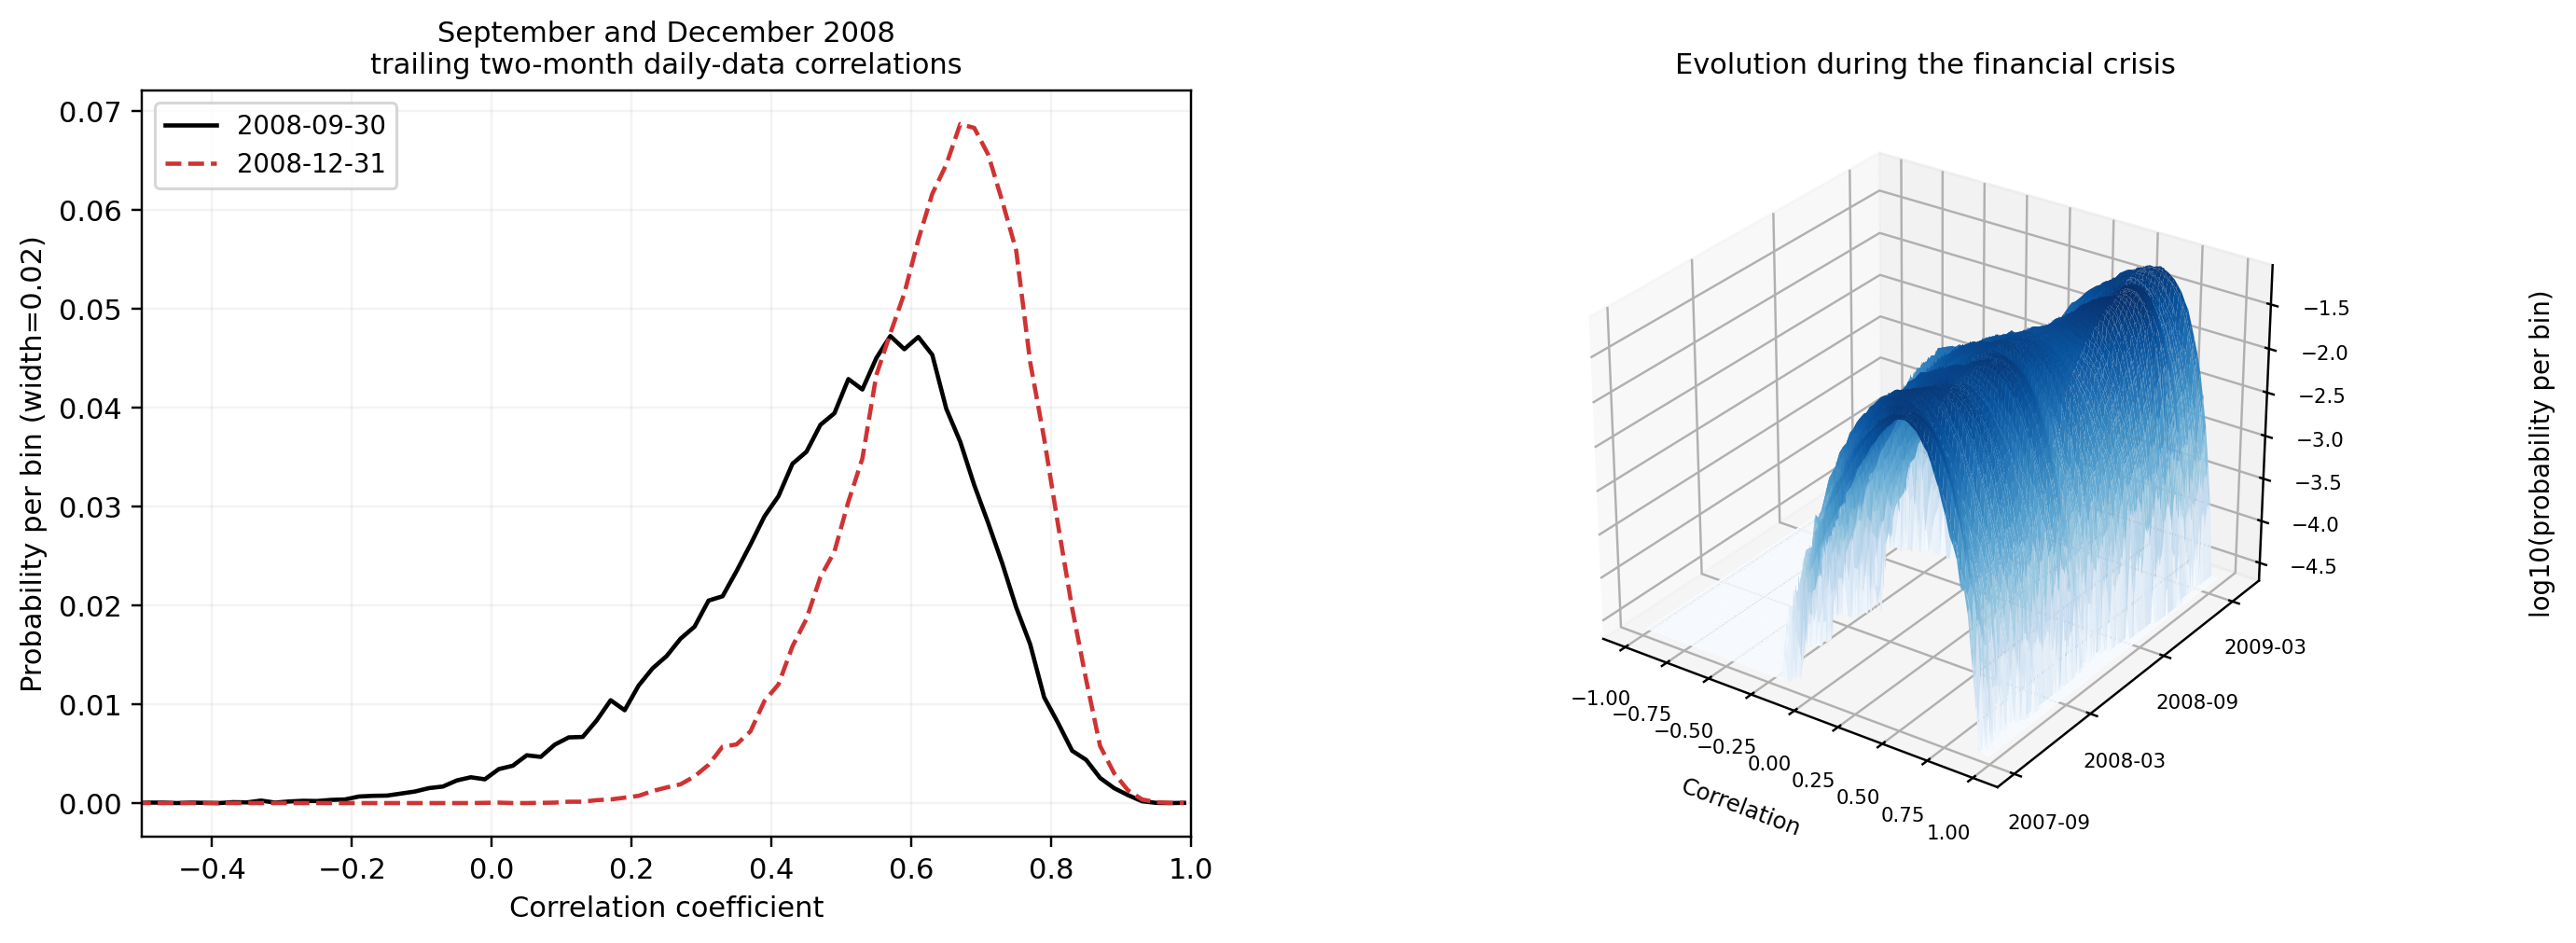
\includegraphics[width=0.98\linewidth]{figure5_crisis_distributions.png}
\caption{Daily trailing-window distribution of stock-pair correlations during the crisis, with histograms for 30 September and 31 December 2008. This is our daily-data counterpart to the article's Figure 5; binning and date choice are explicit implementation decisions.}\label{fig:crisis}
\end{figure}

Figure~\ref{fig:tree} shows the complete fitted tree, with all 114 terms as leaves and boxed nodes marking our eight-state cut. The horizontal scale accumulates child-to-parent center distances, in the spirit of the article's Figure 6.
\begin{figure}[htbp]\centering
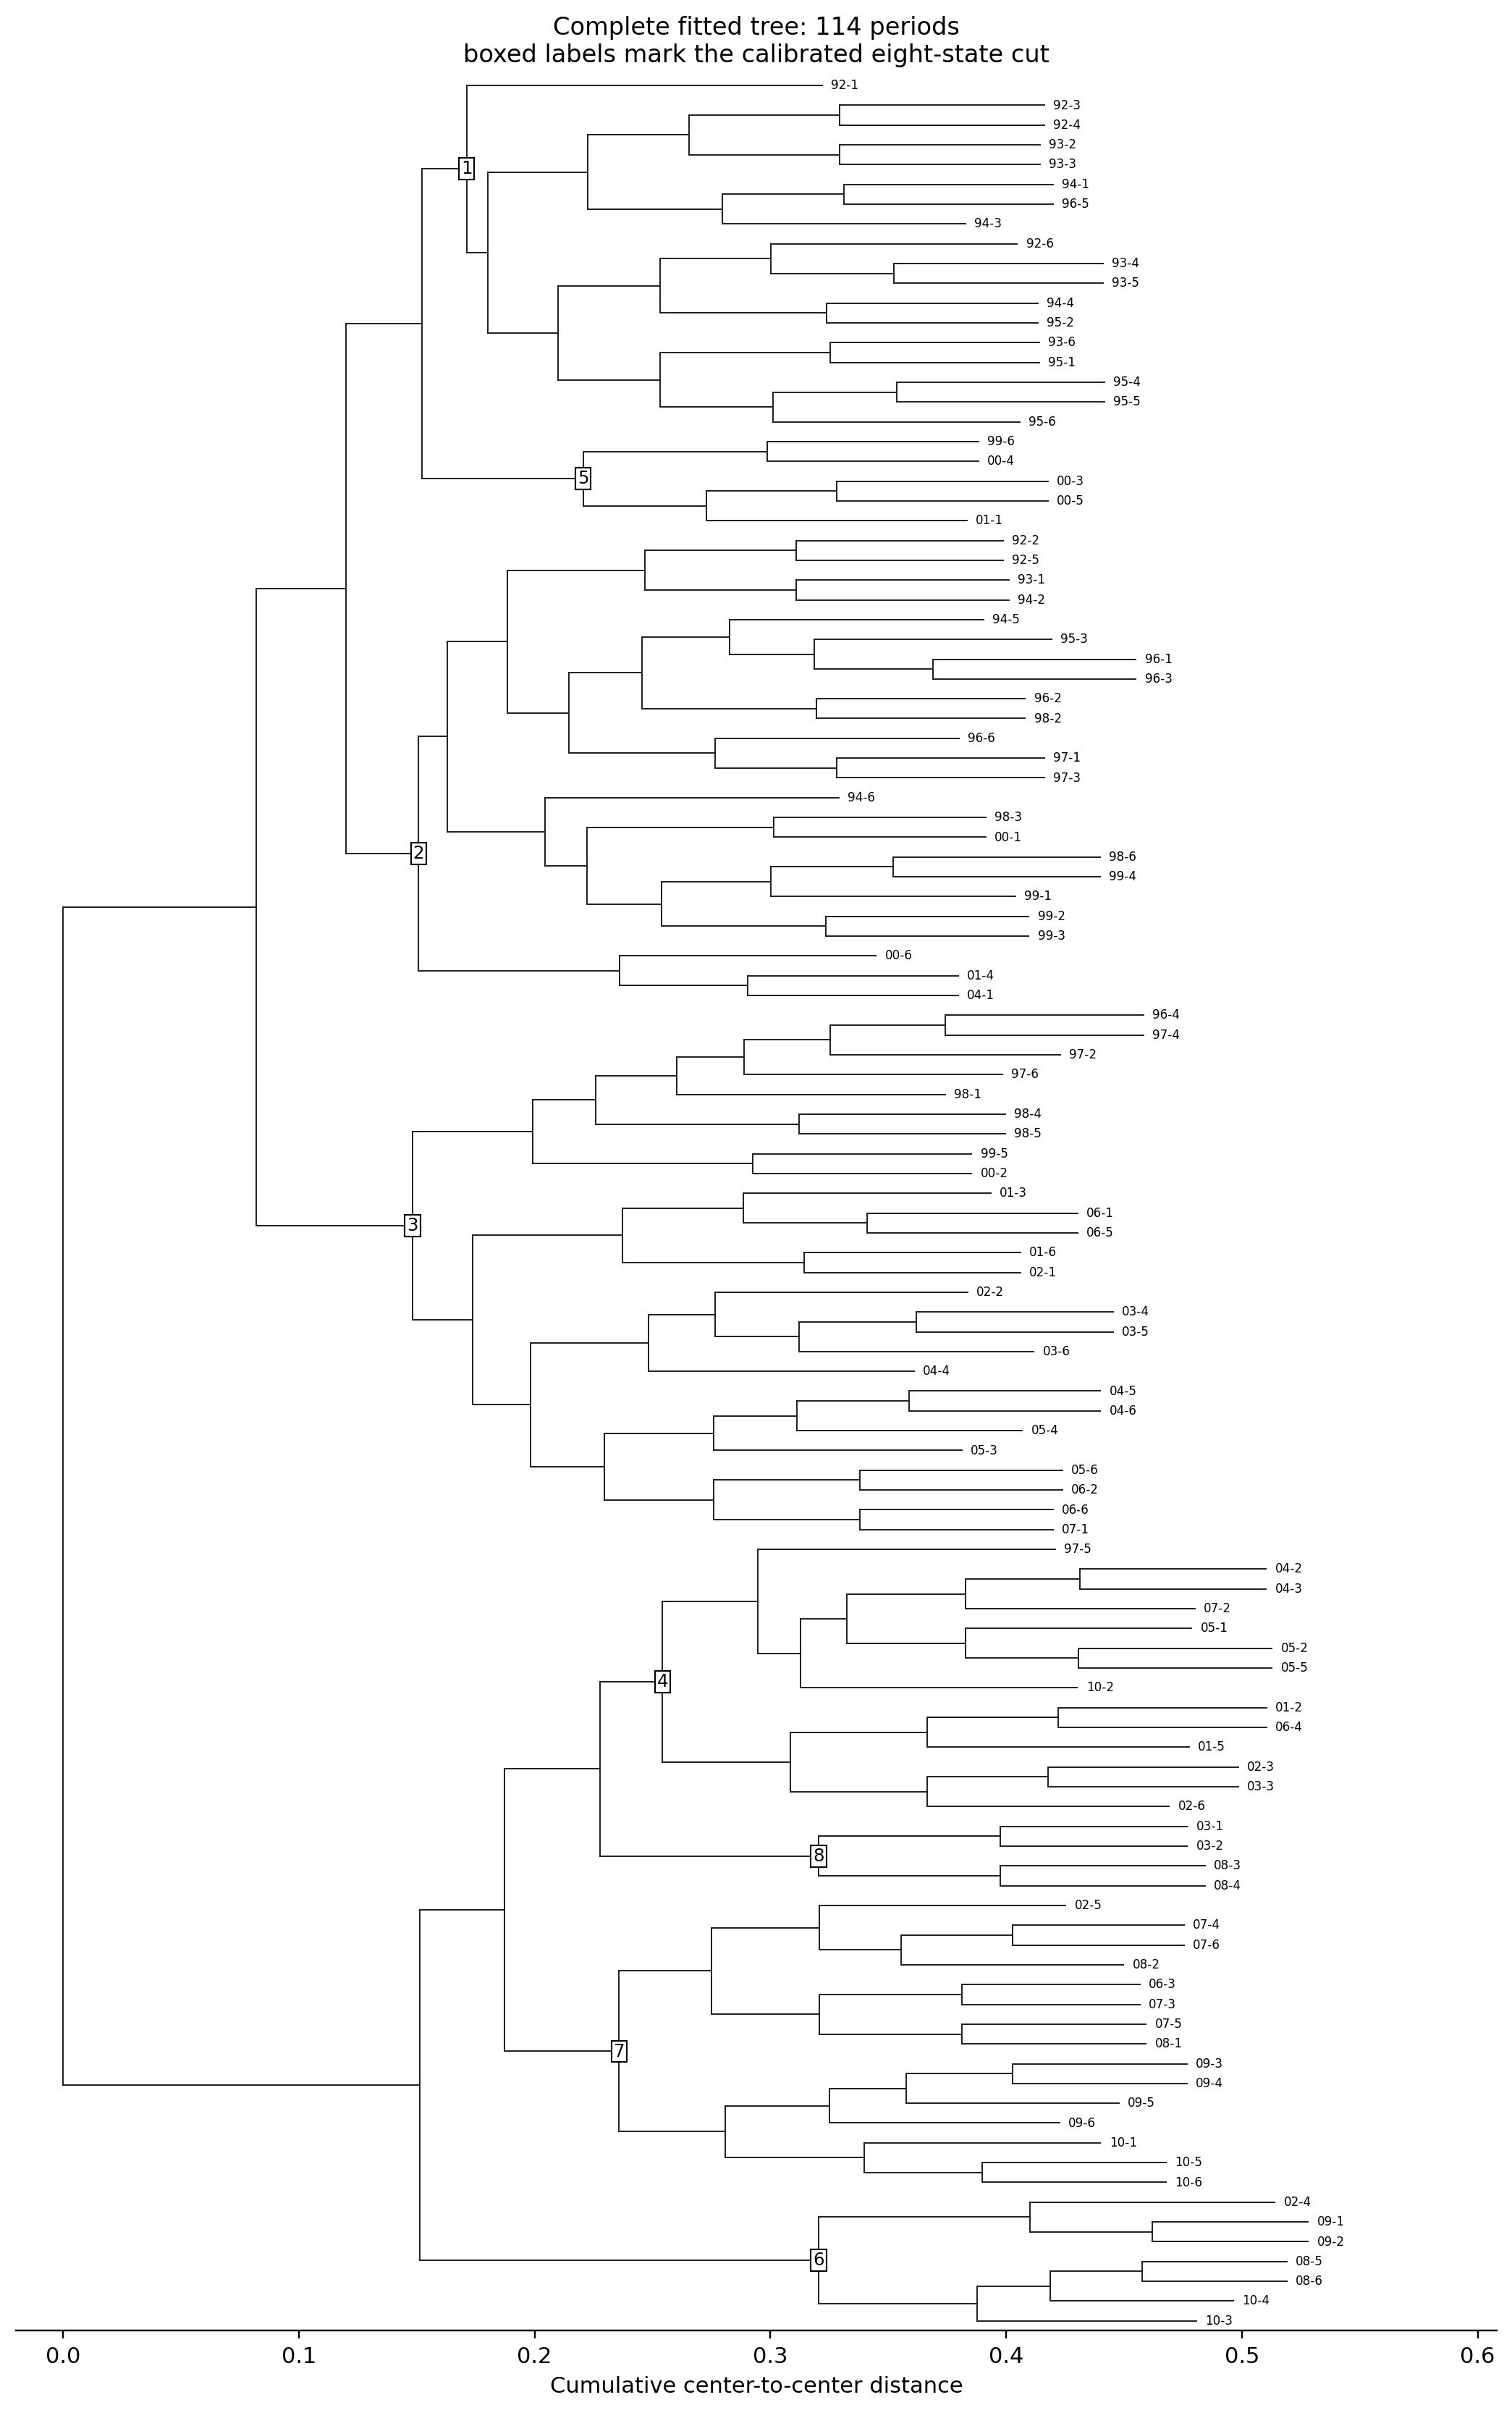
\includegraphics[width=0.90\linewidth]{figure6_complete_tree.png}
\caption{Complete top-down tree to singleton terms. Boxed nodes mark the calibrated eight-state cut; the original article's boxed states come from its own data and threshold.}\label{fig:tree}
\end{figure}

Figure~\ref{fig:eigen} examines the largest eigenvalue of each daily correlation matrix and its absolute difference between dates. Computed eigenvalues range from 22.13 to 211.83. This single number tracks broad collective correlation, but different matrices may have similar largest eigenvalues; it loses sector-specific information.
\begin{figure}[htbp]\centering
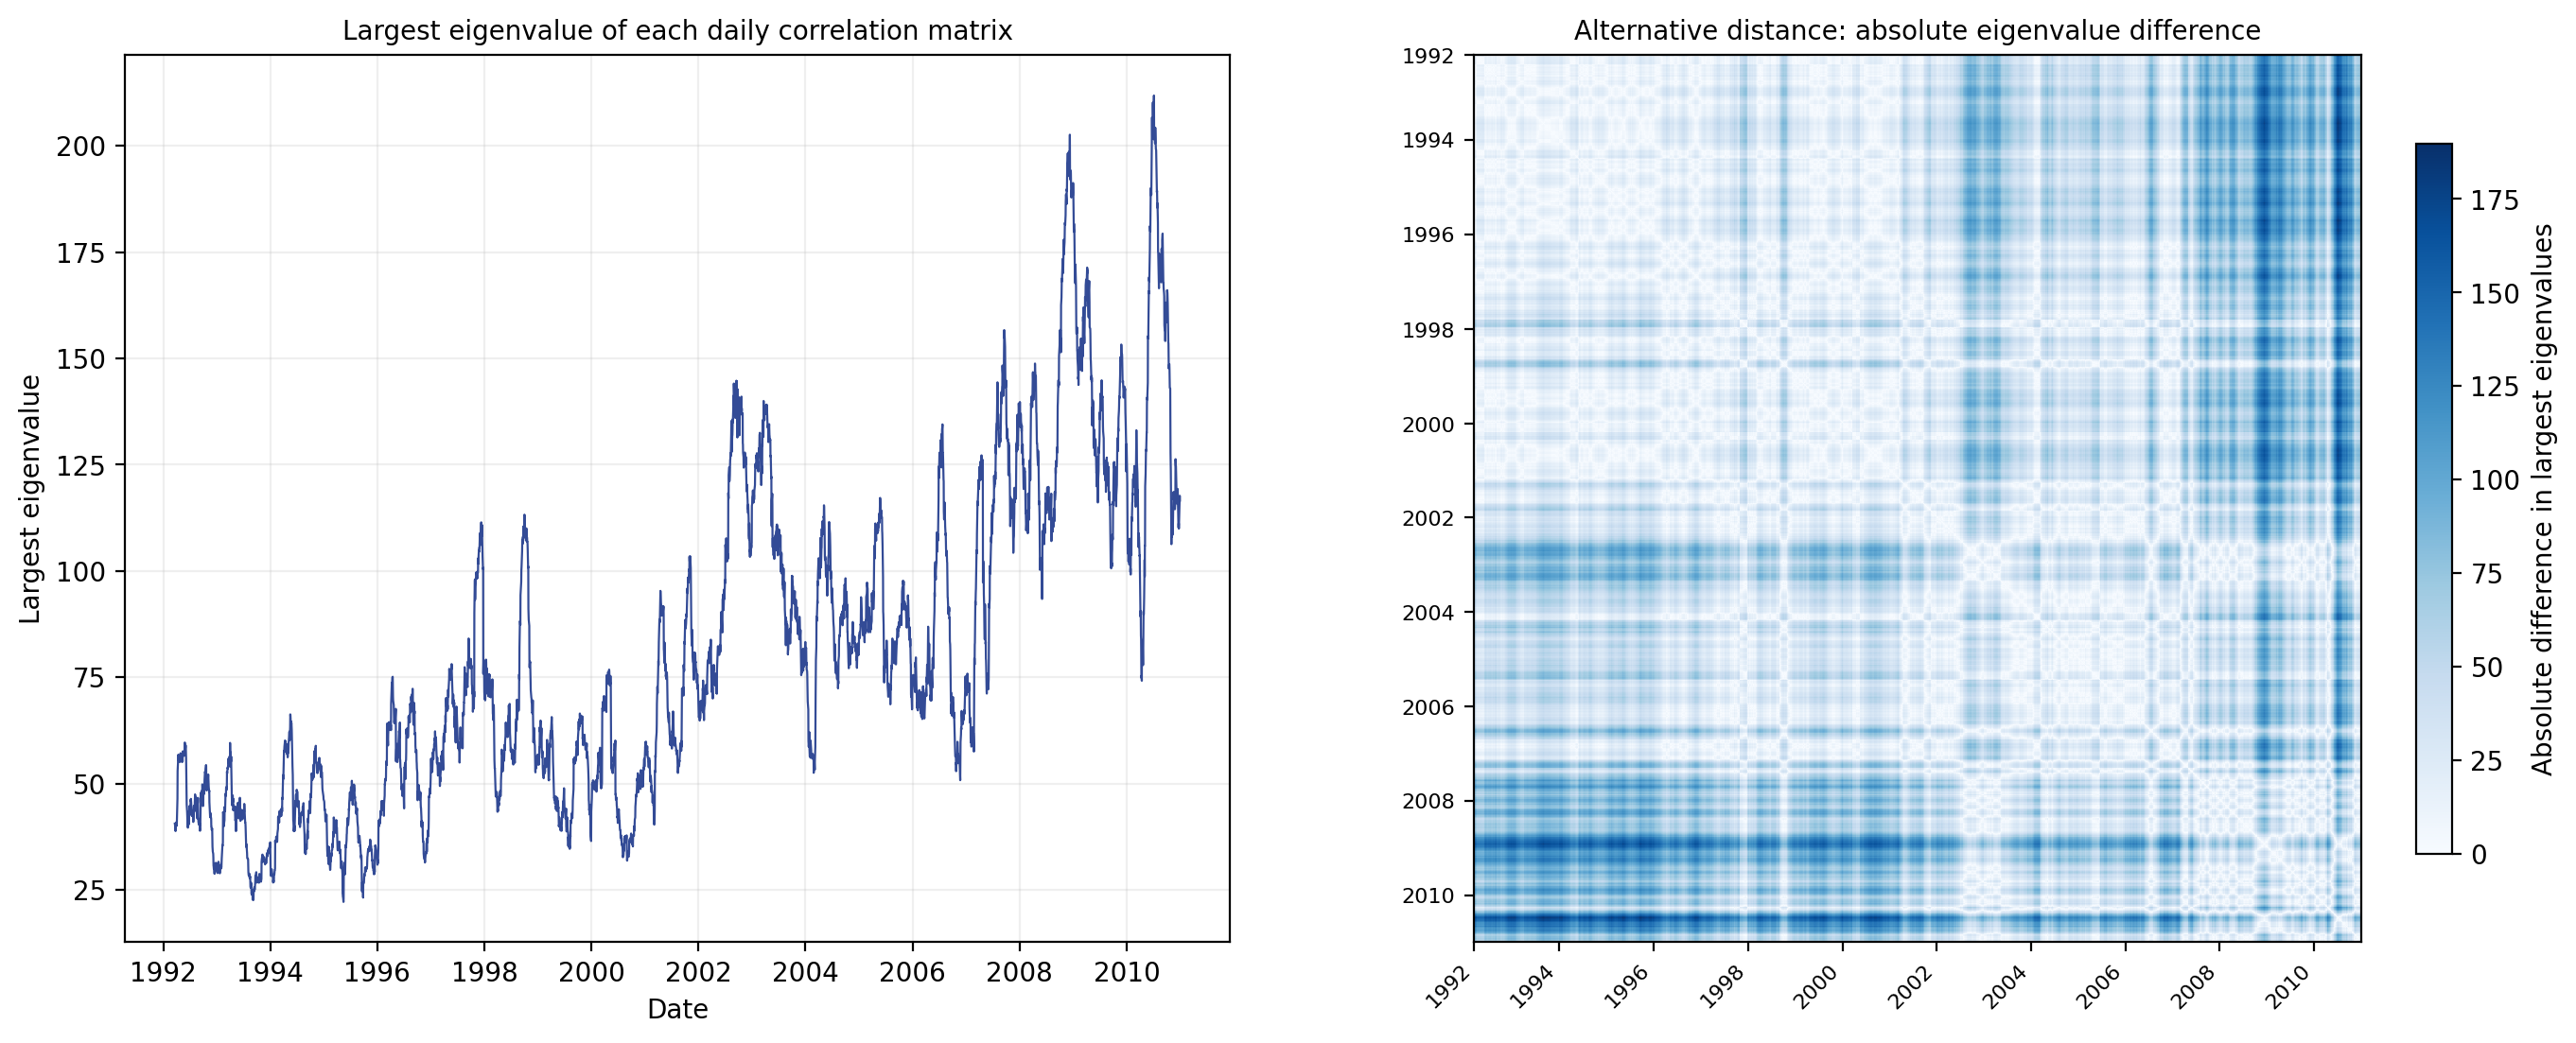
\includegraphics[width=0.94\linewidth]{largest_eigenvalue_alternative.png}
\caption{Largest correlation-matrix eigenvalue over time and pairwise absolute eigenvalue difference, corresponding to the alternative measure discussed in the article.}\label{fig:eigen}
\end{figure}

\FloatBarrier
\section{Comparison with M\"unnix et al.}
\begin{table}[htbp]\centering
\caption{Correspondence and differences between the article and this project.}\label{tab:comparison}
\small\begin{tabularx}{\linewidth}{@{}p{0.23\linewidth}XX@{}}\toprule
Component & Article & This project \\ \midrule
Daily input & Historical S\&P 500 cohort & Supplied adjusted-close files; fixed 296-stock universe after documented exclusions \\
Returns and normalization & Arithmetic returns and 13 recent observations & Same formulas, with explicit zero-variance handling \\
Cluster windows & Disjoint two-month terms & 114 calendar terms, six per year \\
Similarity map & Daily trailing two-month matrices & 4,733 daily trailing windows and all pairwise distances \\
Fine crisis panel & Intraday TAQ, one-hour returns, one-week windows & Daily 2007--2010 zoom; intraday result unavailable \\
Clustering stop & $\tau=0.1465$, eight reported states & Two at $\tau=0.1465$; eight at fitted $\tau=0.1301746$ \\
State figures and tree & Eight centers and full tree & Analogous figures from our dataset and fitted cut \\
\bottomrule\end{tabularx}\end{table}

The central mismatch is the state count at the published threshold. A different stock universe, adjusted-price construction and precision, handling of missing or zero-variance observations, window alignment, or underspecified assignment details may affect the fitted tree. We have not isolated a single cause. Qualitative resemblance in the daily distance maps and crisis correlations is informative, but neither that resemblance nor a forced eight-way cut establishes numerical replication.

The eight-state partition remains useful for exploring sector patterns and threshold sensitivity. Its low mean silhouette, the small sizes of two groups (four and five terms), and its deliberate threshold calibration call for caution before interpreting all eight as independently supported regimes. Silhouette is an internal diagnostic; cluster stability and out-of-sample usefulness remain open questions. The higher score of the two-state cut does not prove global optimality or identify two economic regimes as ground truth.

\section{Reproducibility and repository guide}
The guided Jupyter notebook is \path{notebooks/market_states_paper.ipynb}. It walks through cleaned inputs, returns, normalization, two-month correlation matrices, the complete clustering tree, threshold cuts, state and crisis figures, and daily rolling analysis. The implementation modules in \path{munik/analysis/} are:
\begin{itemize}
\item \path{market_states_numba.py} for matrix distance and clustering;
\item \path{paper_state_figures.py} and \path{paper_remaining_figures.py} for state and crisis graphics;
\item \path{paper_rolling_analysis.py} for daily rolling features and distances;
\item \path{verify_market_states_numba.py} for computation checks.
\end{itemize}
Python dependencies are listed in the repository's \path{requirements.txt}. The images bundled with this report are copies of completed notebook outputs.

The original stock files, large disk-backed arrays, and third-party reference materials are excluded from Git. Readers can inspect the source, notebook, tables, and figures, but reproducing the exact values requires the original CSV files and reference calendar. The older \texttt{run\_pipeline.py} uses an earlier 42-trading-day window schedule and a different split-search configuration; the guided notebook and its helper modules define the results in this report. This distinction matters when rerunning the project.

To reproduce locally, install the packages in \texttt{requirements.txt}, place the original inputs in the directory structure described in the repository README, then execute the notebook cells in order. The full daily pairwise calculation uses approximately 1.84 GB of main feature and distance arrays and is resumable. All numbers reported here come from a completed run, not from a partial progress display.

\section{Conclusions and future work}
This project reconstructs the principal daily-data analysis while exposing consequential cleaning and clustering choices. It finds interpretable changes in stock-correlation structure and a crisis-period shift toward stronger, more uniform positive correlations. Its most informative methodological result is the mismatch in state counts: the article's threshold yields two states on our data, while eight require calibration and exhibit weaker silhouette separation. A requested number of clusters is therefore a result to assess, rather than evidence of a successful reproduction by itself.

The next steps are to verify historical index membership and adjusted-price precision; audit the article's ambiguous clustering notation against any available supplementary detail; measure sensitivity to the stock universe and window construction; and refit the method under joint time-block resampling to assess assignment stability. A further extension could test whether state information improves a specified forecasting or risk task on held-out periods. That would connect descriptive market patterns to the question of when an extracted state is reliable enough to inform a decision.

\begingroup\small
\begin{thebibliography}{9}
\bibitem{munnix2012}
M. C. M\"unnix, T. Shimada, R. Sch\"afer, F. Leyvraz, T. H. Seligman, T. Guhr, and H. E. Stanley, ``Identifying States of a Financial Market,'' \emph{Scientific Reports}, vol. 2, article 644, 2012. \href{https://doi.org/10.1038/srep00644}{doi:10.1038/srep00644}.
\end{thebibliography}
\endgroup
\end{document}
